\PassOptionsToPackage{unicode=true}{hyperref} % options for packages loaded elsewhere
\PassOptionsToPackage{hyphens}{url}
%
\documentclass[]{article}
\usepackage{lmodern}
\usepackage{amssymb,amsmath}
\usepackage{ifxetex,ifluatex}
\usepackage{fixltx2e} % provides \textsubscript
\ifnum 0\ifxetex 1\fi\ifluatex 1\fi=0 % if pdftex
  \usepackage[T1]{fontenc}
  \usepackage[utf8]{inputenc}
  \usepackage{textcomp} % provides euro and other symbols
\else % if luatex or xelatex
  \usepackage{unicode-math}
  \defaultfontfeatures{Ligatures=TeX,Scale=MatchLowercase}
\fi
% use upquote if available, for straight quotes in verbatim environments
\IfFileExists{upquote.sty}{\usepackage{upquote}}{}
% use microtype if available
\IfFileExists{microtype.sty}{%
\usepackage[]{microtype}
\UseMicrotypeSet[protrusion]{basicmath} % disable protrusion for tt fonts
}{}
\IfFileExists{parskip.sty}{%
\usepackage{parskip}
}{% else
\setlength{\parindent}{0pt}
\setlength{\parskip}{6pt plus 2pt minus 1pt}
}
\usepackage{hyperref}
\hypersetup{
            pdftitle={Project 1: Exploratory Data Analysis},
            pdfauthor={Ethan Pieniazek},
            pdfborder={0 0 0},
            breaklinks=true}
\urlstyle{same}  % don't use monospace font for urls
\usepackage[margin=1in]{geometry}
\usepackage{color}
\usepackage{fancyvrb}
\newcommand{\VerbBar}{|}
\newcommand{\VERB}{\Verb[commandchars=\\\{\}]}
\DefineVerbatimEnvironment{Highlighting}{Verbatim}{commandchars=\\\{\}}
% Add ',fontsize=\small' for more characters per line
\usepackage{framed}
\definecolor{shadecolor}{RGB}{248,248,248}
\newenvironment{Shaded}{\begin{snugshade}}{\end{snugshade}}
\newcommand{\AlertTok}[1]{\textcolor[rgb]{0.94,0.16,0.16}{#1}}
\newcommand{\AnnotationTok}[1]{\textcolor[rgb]{0.56,0.35,0.01}{\textbf{\textit{#1}}}}
\newcommand{\AttributeTok}[1]{\textcolor[rgb]{0.77,0.63,0.00}{#1}}
\newcommand{\BaseNTok}[1]{\textcolor[rgb]{0.00,0.00,0.81}{#1}}
\newcommand{\BuiltInTok}[1]{#1}
\newcommand{\CharTok}[1]{\textcolor[rgb]{0.31,0.60,0.02}{#1}}
\newcommand{\CommentTok}[1]{\textcolor[rgb]{0.56,0.35,0.01}{\textit{#1}}}
\newcommand{\CommentVarTok}[1]{\textcolor[rgb]{0.56,0.35,0.01}{\textbf{\textit{#1}}}}
\newcommand{\ConstantTok}[1]{\textcolor[rgb]{0.00,0.00,0.00}{#1}}
\newcommand{\ControlFlowTok}[1]{\textcolor[rgb]{0.13,0.29,0.53}{\textbf{#1}}}
\newcommand{\DataTypeTok}[1]{\textcolor[rgb]{0.13,0.29,0.53}{#1}}
\newcommand{\DecValTok}[1]{\textcolor[rgb]{0.00,0.00,0.81}{#1}}
\newcommand{\DocumentationTok}[1]{\textcolor[rgb]{0.56,0.35,0.01}{\textbf{\textit{#1}}}}
\newcommand{\ErrorTok}[1]{\textcolor[rgb]{0.64,0.00,0.00}{\textbf{#1}}}
\newcommand{\ExtensionTok}[1]{#1}
\newcommand{\FloatTok}[1]{\textcolor[rgb]{0.00,0.00,0.81}{#1}}
\newcommand{\FunctionTok}[1]{\textcolor[rgb]{0.00,0.00,0.00}{#1}}
\newcommand{\ImportTok}[1]{#1}
\newcommand{\InformationTok}[1]{\textcolor[rgb]{0.56,0.35,0.01}{\textbf{\textit{#1}}}}
\newcommand{\KeywordTok}[1]{\textcolor[rgb]{0.13,0.29,0.53}{\textbf{#1}}}
\newcommand{\NormalTok}[1]{#1}
\newcommand{\OperatorTok}[1]{\textcolor[rgb]{0.81,0.36,0.00}{\textbf{#1}}}
\newcommand{\OtherTok}[1]{\textcolor[rgb]{0.56,0.35,0.01}{#1}}
\newcommand{\PreprocessorTok}[1]{\textcolor[rgb]{0.56,0.35,0.01}{\textit{#1}}}
\newcommand{\RegionMarkerTok}[1]{#1}
\newcommand{\SpecialCharTok}[1]{\textcolor[rgb]{0.00,0.00,0.00}{#1}}
\newcommand{\SpecialStringTok}[1]{\textcolor[rgb]{0.31,0.60,0.02}{#1}}
\newcommand{\StringTok}[1]{\textcolor[rgb]{0.31,0.60,0.02}{#1}}
\newcommand{\VariableTok}[1]{\textcolor[rgb]{0.00,0.00,0.00}{#1}}
\newcommand{\VerbatimStringTok}[1]{\textcolor[rgb]{0.31,0.60,0.02}{#1}}
\newcommand{\WarningTok}[1]{\textcolor[rgb]{0.56,0.35,0.01}{\textbf{\textit{#1}}}}
\usepackage{graphicx,grffile}
\makeatletter
\def\maxwidth{\ifdim\Gin@nat@width>\linewidth\linewidth\else\Gin@nat@width\fi}
\def\maxheight{\ifdim\Gin@nat@height>\textheight\textheight\else\Gin@nat@height\fi}
\makeatother
% Scale images if necessary, so that they will not overflow the page
% margins by default, and it is still possible to overwrite the defaults
% using explicit options in \includegraphics[width, height, ...]{}
\setkeys{Gin}{width=\maxwidth,height=\maxheight,keepaspectratio}
\setlength{\emergencystretch}{3em}  % prevent overfull lines
\providecommand{\tightlist}{%
  \setlength{\itemsep}{0pt}\setlength{\parskip}{0pt}}
\setcounter{secnumdepth}{0}
% Redefines (sub)paragraphs to behave more like sections
\ifx\paragraph\undefined\else
\let\oldparagraph\paragraph
\renewcommand{\paragraph}[1]{\oldparagraph{#1}\mbox{}}
\fi
\ifx\subparagraph\undefined\else
\let\oldsubparagraph\subparagraph
\renewcommand{\subparagraph}[1]{\oldsubparagraph{#1}\mbox{}}
\fi

% set default figure placement to htbp
\makeatletter
\def\fps@figure{htbp}
\makeatother


\title{Project 1: Exploratory Data Analysis}
\author{Ethan Pieniazek}
\date{March 15, 2020}

\begin{document}
\maketitle

\emph{After scouring for hours on Kaggle, spreadsheets, and data.gov for
this project in search of two interesting datasets that could be related
by a common variable, I ended up stumbling across some interesting stuff
while not even actively searching. After reading that ``Uncut Gems'' had
the seventh most f-bombs in movie history, I searched along these lines
and found a table on wikipedia that was 144 observations long. The table
included the name and year of the film, rank relative to one another
concerning the total number of f-bombs, total f-bombs, total minutes,
source, and f-bombs per minute. I decided to match this data with
information I found on boxofficemojo.com concerning total domestic box
office gross, director of film, and whether the film was considered a
comedy.}

\emph{After joining by the name of the film I expect to find
associations between the year the film was released and the total amount
of f-bombs used in the film. I also think comedies will on average have
more f-bombs per minute than other genres such as crime drama,
biography, and action films. Comparing how the film did in the box
office with the total f-bombs as well as with directors that had more
than one occurrence in the data also sounds interesting to explore as I
noticed Quentin Tarantino, Martin Scorsese, and Spike Lee were each
found four times throughout the data. Distributing the films equally
into quintiles by year released to then analyze the numeric variables
may reveal the years excessive profanity did not deter the film from
doing poorly in the box office. A big reason this data was interesting
to me is that it made me realize how prevalent data is everywhere, as
there is so much of it freely available to access. It was quite
overwhelming at first, but after I started to focus on finding data
related to an interest of mine, I found it to be not only easier, but
also much more interesting.}

\hypertarget{joining-two-sets-of-data-into-one}{%
\section{Joining Two Sets of Data into
One}\label{joining-two-sets-of-data-into-one}}

\begin{Shaded}
\begin{Highlighting}[]
\KeywordTok{library}\NormalTok{(tidyverse)}
\KeywordTok{library}\NormalTok{(dplyr)}
\NormalTok{films_fbomb <-}\StringTok{ }\KeywordTok{read.csv}\NormalTok{(}\StringTok{"//Users/bitoFLO/Desktop/Website/content/films fbomb.csv"}\NormalTok{, }
    \DataTypeTok{header =}\NormalTok{ T, }\DataTypeTok{na.strings =} \KeywordTok{c}\NormalTok{(}\StringTok{""}\NormalTok{, }\StringTok{"NA"}\NormalTok{))}
\NormalTok{films_domestic_box_ <-}\StringTok{ }\KeywordTok{read.csv}\NormalTok{(}\StringTok{"/Users/bitoFLO/Desktop/Website/content/films domestic box.csv"}\NormalTok{, }
    \DataTypeTok{header =}\NormalTok{ T, }\DataTypeTok{na.strings =} \KeywordTok{c}\NormalTok{(}\StringTok{""}\NormalTok{, }\StringTok{"NA"}\NormalTok{))}
\NormalTok{filmsdata <-}\StringTok{ }\NormalTok{films_fbomb }\OperatorTok\StringTok{ }\KeywordTok{left_join}\NormalTok{(films_domestic_box_, }\DataTypeTok{by =} \KeywordTok{c}\NormalTok{(}\DataTypeTok{film =} \StringTok{"film"}\NormalTok{)) }\OperatorTok\StringTok{ }
\StringTok{    }\KeywordTok{na.omit}\NormalTok{() }\OperatorTok\StringTok{ }\KeywordTok{glimpse}\NormalTok{()}
\end{Highlighting}
\end{Shaded}

\begin{verbatim}
## Observations: 132
## Variables: 9
## $ rank          <int> 3, 4, 5, 6, 7, 8, 9, 10, 11, 12, 13, 14, 15, 16, 17, ...
## $ film          <chr> "The Wolf of Wall Street", "Summer of Sam", "Nil by M...
## $ year          <int> 2013, 1999, 1997, 1995, 2019, 2015, 2007, 2012, 1997,...
## $ fbombs        <int> 569, 435, 428, 422, 408, 392, 367, 326, 318, 315, 313...
## $ minutes       <int> 180, 142, 128, 178, 135, 167, 118, 109, 99, 122, 106,...
## $ source        <fct> SI, PO, SI, FMG, PI, SI, SI, KIM, SI, SI, DR, SI, PO,...
## $ domesticgross <int> 116900694, 19288130, 266130, 42512375, 49929594, 1611...
## $ comedy        <fct> no, no, no, no, no, no, no, no, yes, no, no, yes, no,...
## $ director      <fct> martin.scorsese, spike.lee, gary.oldman, martin.scors...
\end{verbatim}

\emph{I chose to perform a left join because both datasets shared the
common variable `film', but the dataset `films\_domestic\_box\_'
contained three other variables `domesticgross', `director', and
`comedy'. I wanted to join this variable to the `films\_fbombs' dataset
containing the variables `rank', `year', `fbombs', `minutes', and
`source' by the variable both sets shared. 11 cases were dropped after
using na.omit due to NAs found throughout the joined dataset in the
`domesticgross' and `source' columns. I quickly found after knitting
complications that I also needed to specify that the blank cells in each
dataset also constituted as NAs. The problem with dropping NAs is that
important data could be lost, in this case the number 1, 2, 32, 40, 71,
82, etc. ranking films were dropped from further analysis. When
analyzing data with only 144 observations to begin with, losing 8\% of
the data due to NAs is probably not ideal. On the contrary, the reason
the cases were dropped is because there was little to no information
readily available about domestic box office sales, director, or source
where as for all the other films the information was easily found via
boxofficemojo.com. Dropping these cases may have worked to actually make
`filmsdata' more true to the movies that were available to see in
theater, opposed to including some relatively unsuccessful indie films
that also had a great deals of f-bombs.}

\hypertarget{untidying}{%
\section{(Un)tidying}\label{untidying}}

\begin{Shaded}
\begin{Highlighting}[]
\NormalTok{untidyfilms <-}\StringTok{ }\NormalTok{filmsdata }\OperatorTok\StringTok{ }\KeywordTok{pivot_longer}\NormalTok{(}\KeywordTok{contains}\NormalTok{(}\StringTok{"minutes"}\NormalTok{), }
    \DataTypeTok{names_to =} \StringTok{"names"}\NormalTok{, }\DataTypeTok{values_to =} \StringTok{"values"}\NormalTok{) }\OperatorTok\StringTok{ }\KeywordTok{separate}\NormalTok{(director, }
    \DataTypeTok{into =} \KeywordTok{c}\NormalTok{(}\StringTok{"first"}\NormalTok{, }\StringTok{"last"}\NormalTok{))}
\KeywordTok{glimpse}\NormalTok{(untidyfilms)}
\end{Highlighting}
\end{Shaded}

\begin{verbatim}
## Observations: 132
## Variables: 11
## $ rank          <int> 3, 4, 5, 6, 7, 8, 9, 10, 11, 12, 13, 14, 15, 16, 17, ...
## $ film          <chr> "The Wolf of Wall Street", "Summer of Sam", "Nil by M...
## $ year          <int> 2013, 1999, 1997, 1995, 2019, 2015, 2007, 2012, 1997,...
## $ fbombs        <int> 569, 435, 428, 422, 408, 392, 367, 326, 318, 315, 313...
## $ source        <fct> SI, PO, SI, FMG, PI, SI, SI, KIM, SI, SI, DR, SI, PO,...
## $ domesticgross <int> 116900694, 19288130, 266130, 42512375, 49929594, 1611...
## $ comedy        <fct> no, no, no, no, no, no, no, no, yes, no, no, yes, no,...
## $ first         <chr> "martin", "spike", "gary", "martin", "benny", "f", "n...
## $ last          <chr> "scorsese", "lee", "oldman", "scorsese", "safdie", "g...
## $ names         <chr> "minutes", "minutes", "minutes", "minutes", "minutes"...
## $ values        <int> 180, 142, 128, 178, 135, 167, 118, 109, 99, 122, 106,...
\end{verbatim}

\begin{Shaded}
\begin{Highlighting}[]
\NormalTok{untidyfilms }\OperatorTok\StringTok{ }\KeywordTok{pivot_wider}\NormalTok{(}\DataTypeTok{names_from =} \StringTok{"names"}\NormalTok{, }\DataTypeTok{values_from =} \StringTok{"values"}\NormalTok{) }\OperatorTok\StringTok{ }
\StringTok{    }\KeywordTok{unite}\NormalTok{(director, first, last, }\DataTypeTok{sep =} \StringTok{"."}\NormalTok{) }\OperatorTok\StringTok{ }\KeywordTok{glimpse}\NormalTok{()}
\end{Highlighting}
\end{Shaded}

\begin{verbatim}
## Observations: 132
## Variables: 9
## $ rank          <int> 3, 4, 5, 6, 7, 8, 9, 10, 11, 12, 13, 14, 15, 16, 17, ...
## $ film          <chr> "The Wolf of Wall Street", "Summer of Sam", "Nil by M...
## $ year          <int> 2013, 1999, 1997, 1995, 2019, 2015, 2007, 2012, 1997,...
## $ fbombs        <int> 569, 435, 428, 422, 408, 392, 367, 326, 318, 315, 313...
## $ source        <fct> SI, PO, SI, FMG, PI, SI, SI, KIM, SI, SI, DR, SI, PO,...
## $ domesticgross <int> 116900694, 19288130, 266130, 42512375, 49929594, 1611...
## $ comedy        <fct> no, no, no, no, no, no, no, no, yes, no, no, yes, no,...
## $ director      <chr> "martin.scorsese", "spike.lee", "gary.oldman", "marti...
## $ minutes       <int> 180, 142, 128, 178, 135, 167, 118, 109, 99, 122, 106,...
\end{verbatim}

\emph{Often when data is found it is messy, sometimes because it is more
convenient for those collecting data to do so in a wide data format. As
Grolemund and Wickham state; in order to be ``tidy'' each variable needs
its own column, each observation its own row, and each value its own
cell. To make my already tidy data untidy I decided to first use
`pivot\_longer' to make the column title `minutes' go into a new column
called `names' as well as the values to another separate column called
`values'. This expanded the 9 columns my tidy data had to 10 columns
where I then decided to separate `director' into `first' and `last' to
obtain 11 columns. Now that the data looked messy enough, I used the
`pivot\_wider' function to take the names from `names' and the values
from `values' so the minutes column could be brought back along with the
respective lengths of each film. Finally, I used the `unite' function to
bring the director names that were separated into their first name and
last name back into a column titled `director', separating them by a
period for clarity.}

\hypertarget{wrangling-and-generating-summary-statistics}{%
\section{Wrangling and Generating Summary
Statistics}\label{wrangling-and-generating-summary-statistics}}

\hypertarget{section}{%
\subsubsection{1.}\label{section}}

\begin{Shaded}
\begin{Highlighting}[]
\NormalTok{filmsdata <-}\StringTok{ }\NormalTok{filmsdata }\OperatorTok\StringTok{ }\KeywordTok{mutate}\NormalTok{(}\DataTypeTok{fbombspermin =}\NormalTok{ fbombs}\OperatorTok{/}\NormalTok{minutes)}
\NormalTok{filmsdata }\OperatorTok\StringTok{ }\KeywordTok{filter}\NormalTok{(year }\OperatorTok{<}\StringTok{ }\DecValTok{2000}\NormalTok{) }\OperatorTok\StringTok{ }\KeywordTok{summarize}\NormalTok{(}\DataTypeTok{avg_fbombspermin =} \KeywordTok{mean}\NormalTok{(fbombspermin), }
    \DataTypeTok{avg_minutes =} \KeywordTok{mean}\NormalTok{(minutes))}
\end{Highlighting}
\end{Shaded}

\begin{verbatim}
##   avg_fbombspermin avg_minutes
## 1         1.873157    119.9792
\end{verbatim}

\begin{Shaded}
\begin{Highlighting}[]
\NormalTok{filmsdata }\OperatorTok\StringTok{ }\KeywordTok{filter}\NormalTok{(year }\OperatorTok{>=}\StringTok{ }\DecValTok{2000}\NormalTok{) }\OperatorTok\StringTok{ }\KeywordTok{summarize}\NormalTok{(}\DataTypeTok{avg_fbombspermin =} \KeywordTok{mean}\NormalTok{(fbombspermin), }
    \DataTypeTok{avg_minutes =} \KeywordTok{mean}\NormalTok{(minutes))}
\end{Highlighting}
\end{Shaded}

\begin{verbatim}
##   avg_fbombspermin avg_minutes
## 1         1.896294    112.4762
\end{verbatim}

\hypertarget{section-1}{%
\subsubsection{2.}\label{section-1}}

\begin{Shaded}
\begin{Highlighting}[]
\NormalTok{filmsdata }\OperatorTok\StringTok{ }\KeywordTok{group_by}\NormalTok{(film, director, year) }\OperatorTok\StringTok{ }\KeywordTok{select}\NormalTok{(fbombspermin, }
\NormalTok{    fbombs) }\OperatorTok\StringTok{ }\KeywordTok{summarize}\NormalTok{(}\DataTypeTok{avg_fbombspermin =} \KeywordTok{mean}\NormalTok{(fbombspermin), }
    \DataTypeTok{total_fbombs =} \KeywordTok{sum}\NormalTok{(fbombs)) }\OperatorTok\StringTok{ }\KeywordTok{arrange}\NormalTok{(director) }\OperatorTok\StringTok{ }\KeywordTok{glimpse}\NormalTok{()}
\end{Highlighting}
\end{Shaded}

\begin{verbatim}
## Observations: 132
## Variables: 5
## Groups: film, director [132]
## $ film             <chr> "The Commitments", "Dead Presidents", "Menace II S...
## $ director         <fct> alan.parker, albert.hughes, albert.hughes, andrea....
## $ year             <int> 1991, 1995, 1993, 2016, 2012, 2010, 2010, 2000, 20...
## $ avg_fbombspermin <dbl> 1.4322034, 1.3193277, 3.1122449, 0.9202454, 1.9896...
## $ total_fbombs     <int> 169, 157, 305, 150, 193, 270, 155, 153, 210, 193, ...
\end{verbatim}

\hypertarget{section-2}{%
\subsubsection{3.}\label{section-2}}

\begin{Shaded}
\begin{Highlighting}[]
\NormalTok{filmsdata }\OperatorTok\StringTok{ }\KeywordTok{group_by}\NormalTok{(comedy) }\OperatorTok\StringTok{ }\KeywordTok{select}\NormalTok{(domesticgross, fbombs) }\OperatorTok\StringTok{ }
\StringTok{    }\KeywordTok{summarize}\NormalTok{(}\DataTypeTok{avg_domesticgross =} \KeywordTok{mean}\NormalTok{(domesticgross), }\DataTypeTok{sd_domesticgross =} \KeywordTok{sd}\NormalTok{(domesticgross), }
        \DataTypeTok{avg_fbombs =} \KeywordTok{mean}\NormalTok{(fbombs))}
\end{Highlighting}
\end{Shaded}

\begin{verbatim}
## # A tibble: 2 x 4
##   comedy avg_domesticgross sd_domesticgross avg_fbombs
##   <fct>              <dbl>            <dbl>      <dbl>
## 1 no             32480571.        41259813.       225.
## 2 yes            36732615.        44822150.       194.
\end{verbatim}

\hypertarget{section-3}{%
\subsubsection{4.}\label{section-3}}

\begin{Shaded}
\begin{Highlighting}[]
\NormalTok{filmsdata }\OperatorTok\StringTok{ }\KeywordTok{mutate}\NormalTok{(}\DataTypeTok{quintileyr =} \KeywordTok{cut}\NormalTok{(filmsdata}\OperatorTok{$}\NormalTok{year, }\KeywordTok{quantile}\NormalTok{(filmsdata}\OperatorTok{$}\NormalTok{year, }
    \DecValTok{0}\OperatorTok{:}\DecValTok{5}\OperatorTok{/}\DecValTok{5}\NormalTok{), }\DataTypeTok{include.lowest =}\NormalTok{ T)) }\OperatorTok\StringTok{ }\KeywordTok{group_by}\NormalTok{(quintileyr) }\OperatorTok\StringTok{ }
\StringTok{    }\KeywordTok{summarize}\NormalTok{(}\DataTypeTok{avg_fbombs =} \KeywordTok{mean}\NormalTok{(fbombs), }\DataTypeTok{var_fbombs =} \KeywordTok{var}\NormalTok{(fbombs))}
\end{Highlighting}
\end{Shaded}

\begin{verbatim}
## # A tibble: 5 x 3
##   quintileyr  avg_fbombs var_fbombs
##   <fct>            <dbl>      <dbl>
## 1 [1978,1997]       216.      5287.
## 2 (1997,2000]       210.      3883.
## 3 (2000,2006]       224.      3288.
## 4 (2006,2012]       203.      3563.
## 5 (2012,2019]       208.     10071.
\end{verbatim}

\begin{Shaded}
\begin{Highlighting}[]
\NormalTok{filmsdata <-}\StringTok{ }\NormalTok{filmsdata }\OperatorTok\StringTok{ }\KeywordTok{mutate}\NormalTok{(}\DataTypeTok{quintileyr =} \KeywordTok{cut}\NormalTok{(filmsdata}\OperatorTok{$}\NormalTok{year, }
    \KeywordTok{quantile}\NormalTok{(filmsdata}\OperatorTok{$}\NormalTok{year, }\DecValTok{0}\OperatorTok{:}\DecValTok{5}\OperatorTok{/}\DecValTok{5}\NormalTok{), }\DataTypeTok{include.lowest =}\NormalTok{ T))}
\end{Highlighting}
\end{Shaded}

\hypertarget{section-4}{%
\subsubsection{5.}\label{section-4}}

\begin{Shaded}
\begin{Highlighting}[]
\NormalTok{filmsdata }\OperatorTok\StringTok{ }\KeywordTok{summarize}\NormalTok{(}\DataTypeTok{distinct_year_count =} \KeywordTok{n_distinct}\NormalTok{(year), }
    \DataTypeTok{distinct_source_count =} \KeywordTok{n_distinct}\NormalTok{(source), }\DataTypeTok{distinct_director_count =} \KeywordTok{n_distinct}\NormalTok{(director))}
\end{Highlighting}
\end{Shaded}

\begin{verbatim}
##   distinct_year_count distinct_source_count distinct_director_count
## 1                  36                    10                     107
\end{verbatim}

\hypertarget{section-5}{%
\subsubsection{6.}\label{section-5}}

\begin{Shaded}
\begin{Highlighting}[]
\NormalTok{filmsdata }\OperatorTok\StringTok{ }\KeywordTok{group_by}\NormalTok{(quintileyr) }\OperatorTok\StringTok{ }\KeywordTok{summarize}\NormalTok{(}\DataTypeTok{correlation =} \KeywordTok{cor}\NormalTok{(fbombs, }
\NormalTok{    minutes))}
\end{Highlighting}
\end{Shaded}

\begin{verbatim}
## # A tibble: 5 x 2
##   quintileyr  correlation
##   <fct>             <dbl>
## 1 [1978,1997]      0.105 
## 2 (1997,2000]      0.327 
## 3 (2000,2006]      0.0912
## 4 (2006,2012]     -0.0923
## 5 (2012,2019]      0.657
\end{verbatim}

\hypertarget{section-6}{%
\subsubsection{7.}\label{section-6}}

\begin{Shaded}
\begin{Highlighting}[]
\NormalTok{filmsdata }\OperatorTok\StringTok{ }\KeywordTok{group_by}\NormalTok{(source) }\OperatorTok\StringTok{ }\KeywordTok{summarize}\NormalTok{(}\DataTypeTok{min_domesticgross =} \KeywordTok{min}\NormalTok{(domesticgross), }
    \DataTypeTok{max_domesticgross =} \KeywordTok{max}\NormalTok{(domesticgross)) }\OperatorTok\StringTok{ }\KeywordTok{arrange}\NormalTok{(}\KeywordTok{desc}\NormalTok{(max_domesticgross))}
\end{Highlighting}
\end{Shaded}

\begin{verbatim}
## # A tibble: 10 x 3
##    source min_domesticgross max_domesticgross
##    <fct>              <int>             <int>
##  1 PI                141396         191719337
##  2 SI                127923         161197785
##  3 KIM                15843         159582188
##  4 FMG                 2942         140539099
##  5 IMDb           115646235         115646235
##  6 PO                104257          27912072
##  7 SD              27545445          27545445
##  8 TFF              6521083           6521083
##  9 DR                316319            316319
## 10 MR                139692            139692
\end{verbatim}

\hypertarget{section-7}{%
\subsubsection{8.}\label{section-7}}

\begin{Shaded}
\begin{Highlighting}[]
\NormalTok{filmsdata }\OperatorTok\StringTok{ }\KeywordTok{select}\NormalTok{(}\OperatorTok{-}\NormalTok{rank, }\OperatorTok{-}\NormalTok{film, }\OperatorTok{-}\NormalTok{year, }\OperatorTok{-}\NormalTok{source, }\OperatorTok{-}\NormalTok{comedy, }\OperatorTok{-}\NormalTok{director, }
    \OperatorTok{-}\NormalTok{quintileyr) }\OperatorTok\StringTok{ }\KeywordTok{cor}\NormalTok{()}
\end{Highlighting}
\end{Shaded}

\begin{verbatim}
##                     fbombs    minutes domesticgross fbombspermin
## fbombs         1.000000000  0.2458415  -0.005275904    0.8068090
## minutes        0.245841489  1.0000000   0.258155168   -0.3346682
## domesticgross -0.005275904  0.2581552   1.000000000   -0.2139089
## fbombspermin   0.806808988 -0.3346682  -0.213908912    1.0000000
\end{verbatim}

\hypertarget{section-8}{%
\subsubsection{9.}\label{section-8}}

\begin{Shaded}
\begin{Highlighting}[]
\NormalTok{top10comedies <-}\StringTok{ }\NormalTok{filmsdata }\OperatorTok\StringTok{ }\KeywordTok{filter}\NormalTok{(comedy }\OperatorTok{==}\StringTok{ "yes"}\NormalTok{) }\OperatorTok\StringTok{ }\KeywordTok{group_by}\NormalTok{(film, }
\NormalTok{    rank) }\OperatorTok\StringTok{ }\KeywordTok{select}\NormalTok{(fbombspermin, fbombs, rank, domesticgross) }\OperatorTok\StringTok{ }
\StringTok{    }\KeywordTok{summarize}\NormalTok{(fbombs, fbombspermin, domesticgross) }\OperatorTok\StringTok{ }\KeywordTok{arrange}\NormalTok{(rank) }\OperatorTok\StringTok{ }
\StringTok{    }\KeywordTok{filter}\NormalTok{(rank }\OperatorTok{<=}\StringTok{ }\DecValTok{45}\NormalTok{)}
\NormalTok{top10noncomedies <-}\StringTok{ }\NormalTok{filmsdata }\OperatorTok\StringTok{ }\KeywordTok{filter}\NormalTok{(comedy }\OperatorTok{==}\StringTok{ "no"}\NormalTok{) }\OperatorTok\StringTok{ }
\StringTok{    }\KeywordTok{group_by}\NormalTok{(film, rank) }\OperatorTok\StringTok{ }\KeywordTok{select}\NormalTok{(fbombspermin, fbombs, rank, }
\NormalTok{    domesticgross) }\OperatorTok\StringTok{ }\KeywordTok{summarize}\NormalTok{(fbombs, fbombspermin, domesticgross) }\OperatorTok\StringTok{ }
\StringTok{    }\KeywordTok{arrange}\NormalTok{(rank) }\OperatorTok\StringTok{ }\KeywordTok{filter}\NormalTok{(rank }\OperatorTok{<=}\StringTok{ }\DecValTok{13}\NormalTok{)}
\NormalTok{top10comedies}
\end{Highlighting}
\end{Shaded}

\begin{verbatim}
## # A tibble: 10 x 5
## # Groups:   film [10]
##    film                             rank fbombs fbombspermin domesticgross
##    <chr>                           <int>  <int>        <dbl>         <int>
##  1 Twin Town                          11    318         3.21        127923
##  2 Martin Lawrence Live: Runteldat    14    311         2.75      19184820
##  3 Made                               19    291         3.10       5313300
##  4 I'm Still Here                     23    280         2.62        408983
##  5 The Big Lebowski                   29    260         2.22      18034458
##  6 Jay and Silent Bob Strike Back     30    248         2.38      30085147
##  7 Do the Right Thing                 33    240         2         27545445
##  8 Goon                               40    231         2.48       4168528
##  9 Gridlock'd                         43    227         2.49       5571205
## 10 Eddie Murphy Raw                   45    223         2.48      50504655
\end{verbatim}

\begin{Shaded}
\begin{Highlighting}[]
\NormalTok{top10noncomedies}
\end{Highlighting}
\end{Shaded}

\begin{verbatim}
## # A tibble: 10 x 5
## # Groups:   film [10]
##    film                     rank fbombs fbombspermin domesticgross
##    <chr>                   <int>  <int>        <dbl>         <int>
##  1 The Wolf of Wall Street     3    569         3.16     116900694
##  2 Summer of Sam               4    435         3.06      19288130
##  3 Nil by Mouth                5    428         3.34        266130
##  4 Casino                      6    422         2.37      42512375
##  5 Uncut Gems                  7    408         3.02      49929594
##  6 Straight Outta Compton      8    392         2.35     161197785
##  7 Alpha Dog                   9    367         3.11      15309602
##  8 End of Watch               10    326         2.99      41003371
##  9 Running Scared             12    315         2.58       6855137
## 10 Sweet Sixteen              13    313         2.95        316319
\end{verbatim}

\hypertarget{section-9}{%
\subsubsection{10.}\label{section-9}}

\begin{Shaded}
\begin{Highlighting}[]
\NormalTok{filmsdata }\OperatorTok\StringTok{ }\KeywordTok{group_by}\NormalTok{(director) }\OperatorTok\StringTok{ }\KeywordTok{mutate}\NormalTok{(}\DataTypeTok{directorappearances =} \KeywordTok{n}\NormalTok{()) }\OperatorTok\StringTok{ }
\StringTok{    }\KeywordTok{filter}\NormalTok{(directorappearances }\OperatorTok{>=}\StringTok{ }\DecValTok{2}\NormalTok{) }\OperatorTok\StringTok{ }\KeywordTok{group_by}\NormalTok{(director, directorappearances) }\OperatorTok\StringTok{ }
\StringTok{    }\KeywordTok{select}\NormalTok{(director, directorappearances) }\OperatorTok\StringTok{ }\KeywordTok{summarize}\NormalTok{() }\OperatorTok\StringTok{ }
\StringTok{    }\KeywordTok{arrange}\NormalTok{(}\KeywordTok{desc}\NormalTok{(directorappearances))}
\end{Highlighting}
\end{Shaded}

\begin{verbatim}
## # A tibble: 17 x 2
## # Groups:   director [17]
##    director             directorappearances
##    <fct>                              <int>
##  1 martin.scorsese                        4
##  2 quentin.tarantino                      4
##  3 spike.lee                              4
##  4 david.ayer                             3
##  5 kevin.smith                            3
##  6 albert.hughes                          2
##  7 benny.boom                             2
##  8 benny.safdie                           2
##  9 damon.dash                             2
## 10 jim.sheridan                           2
## 11 joe.carnahan                           2
## 12 joel.schumacher                        2
## 13 ken.loach                              2
## 14 larry.clark                            2
## 15 oliver.stone                           2
## 16 paul.thomas.anderson                   2
## 17 peter.berg                             2
\end{verbatim}

\begin{Shaded}
\begin{Highlighting}[]
\NormalTok{filmsdata <-}\StringTok{ }\NormalTok{filmsdata }\OperatorTok\StringTok{ }\KeywordTok{group_by}\NormalTok{(director) }\OperatorTok\StringTok{ }\KeywordTok{mutate}\NormalTok{(}\DataTypeTok{directorappearances =} \KeywordTok{n}\NormalTok{()) }\OperatorTok\StringTok{ }
\StringTok{    }\NormalTok{ungroup}
\end{Highlighting}
\end{Shaded}

\emph{By using the six core dplyr functions, it made it easy to
manipulate and explore the joined dataset. For films between 1978 and
1999 the average f-bombs per minute was 1.873157 and the average length
of film was 119.9792 minutes. Films between 2000 and 2019 showed an
average `fbombspermin' being slightly greater with a value of 1.896294
while the length of film was generally shorter at 112.4762 minutes on
average. Grouping the data by film, director, and year made summarizing
the average `fbombspermin' and total `fbombs' for each film concise. I
then grouped the data by `comedy' to give the the `avg\_domesticgross',
`sd\_domesticgross', and `avg\_fbombs' for the comedies and
non-comedies, on average the comedies bringing in more revenue while
having fewer f-bombs (not what I hypothesized). The `quintileyr'
variable was mutated to sort the films into five equal quintiles based
on year released, showing the average f-bomb count to be higher in the
first three quintiles than the most recent two, which was surprising
considering how it feels the world has been more desensitized to
profanity when compared to 30 years ago. Using the `cor' function with
the newly mutated `quintileyr' revealed the strongest linear
relationship between f-bombs and length was in the last quintile
(2013-2019).}

\emph{Summarizing with 'n\_distinct' revealed there were 36 distinct
years, 10 distinct sources, and 107 distinct directors in the data.
`Plugged In' was the source sited with the highest recorded domestic
gross sales for a film (``22 Jump Street'') while `Family Media Group'
was sited for one that had the lowest domestic gross sales (``Ash
Wednesday''). The correlation matrix summarized the data showing the
highest correlation existed between `fbombs' and `fbombspermin'.
Filtering the comedies and non-comedies and then filtering by rank gave
way to two cool new data sets, showing the top 10 ranked comedies for
f-bomb count and the top 10 ranked non-comedies for f-bomb count. ``Twin
Tower'' took the cake for being the comedy with the most f-bombs (318
f-bombs) while ``The Wolf of Wall Street'' had the most for a non-comedy
(569 f-bombs). The last summary statistic I created was interesting
because it mutated a new function (`directorappearances') to then
summarize and arrange the directors who appeared multiple times in the
data set. This was particularly useful for making my first plot.}

\hypertarget{correlation-heapmap-of-numeric-variables}{%
\section{Correlation Heapmap of Numeric
Variables}\label{correlation-heapmap-of-numeric-variables}}

\begin{Shaded}
\begin{Highlighting}[]
\KeywordTok{library}\NormalTok{(reshape2)}
\NormalTok{filmsdata_cormatrix <-}\StringTok{ }\NormalTok{filmsdata }\OperatorTok\StringTok{ }\NormalTok{ungroup }\OperatorTok\StringTok{ }\KeywordTok{select}\NormalTok{(}\OperatorTok{-}\NormalTok{rank, }
    \OperatorTok{-}\NormalTok{film, }\OperatorTok{-}\NormalTok{year, }\OperatorTok{-}\NormalTok{source, }\OperatorTok{-}\NormalTok{comedy, }\OperatorTok{-}\NormalTok{director, }\OperatorTok{-}\NormalTok{quintileyr, }\OperatorTok{-}\NormalTok{directorappearances) }\OperatorTok\StringTok{ }
\StringTok{    }\KeywordTok{cor}\NormalTok{()}
\NormalTok{melt_cormatrix <-}\StringTok{ }\KeywordTok{melt}\NormalTok{(filmsdata_cormatrix)}
\KeywordTok{ggplot}\NormalTok{(}\DataTypeTok{data =}\NormalTok{ melt_cormatrix, }\KeywordTok{aes}\NormalTok{(}\DataTypeTok{x =}\NormalTok{ Var1, }\DataTypeTok{y =}\NormalTok{ Var2, }\DataTypeTok{fill =}\NormalTok{ value)) }\OperatorTok{+}\StringTok{ }
\StringTok{    }\KeywordTok{geom_tile}\NormalTok{(}\DataTypeTok{color =} \StringTok{"white"}\NormalTok{) }\OperatorTok{+}\StringTok{ }\KeywordTok{scale_fill_gradient2}\NormalTok{(}\DataTypeTok{low =} \StringTok{"yellow"}\NormalTok{, }
    \DataTypeTok{high =} \StringTok{"orange"}\NormalTok{, }\DataTypeTok{mid =} \StringTok{"white"}\NormalTok{, }\DataTypeTok{midpoint =} \DecValTok{0}\NormalTok{, }\DataTypeTok{limit =} \KeywordTok{c}\NormalTok{(}\OperatorTok{-}\DecValTok{1}\NormalTok{, }
        \DecValTok{1}\NormalTok{), }\DataTypeTok{space =} \StringTok{"Lab"}\NormalTok{, }\DataTypeTok{name =} \StringTok{"Correlation"}\NormalTok{) }\OperatorTok{+}\StringTok{ }\KeywordTok{theme_minimal}\NormalTok{() }\OperatorTok{+}\StringTok{ }
\StringTok{    }\KeywordTok{theme}\NormalTok{(}\DataTypeTok{axis.text.x =} \KeywordTok{element_text}\NormalTok{(}\DataTypeTok{angle =} \DecValTok{30}\NormalTok{, }\DataTypeTok{vjust =} \DecValTok{1}\NormalTok{, }\DataTypeTok{size =} \DecValTok{9}\NormalTok{, }
        \DataTypeTok{hjust =} \FloatTok{0.7}\NormalTok{)) }\OperatorTok{+}\StringTok{ }\KeywordTok{coord_fixed}\NormalTok{() }\OperatorTok{+}\StringTok{ }\KeywordTok{ggtitle}\NormalTok{(}\StringTok{"Correlation heatmap of numeric variables"}\NormalTok{) }\OperatorTok{+}\StringTok{ }
\StringTok{    }\KeywordTok{theme}\NormalTok{(}\DataTypeTok{plot.title =} \KeywordTok{element_text}\NormalTok{(}\DataTypeTok{hjust =} \FloatTok{0.5}\NormalTok{))}
\end{Highlighting}
\end{Shaded}

\begin{center}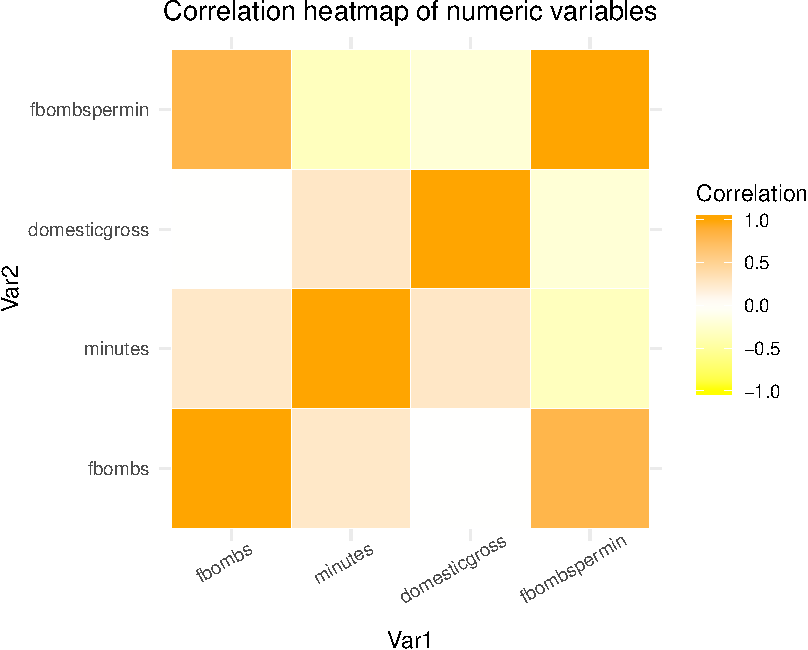
\includegraphics{project1.ethanpieniazekweb_files/figure-latex/unnamed-chunk-13-1} \end{center}

\emph{This correlation heatmap takes the correlation matrix coded for
summary statistic \#8 and converts it into a visualization that makes it
easier to see the relationships between the numeric variables. The most
positive correlation is shown between `fbombs' and `fbombspermin' while
the most negative is shown between `minutes' and `fbombspermin'. It was
important to use the dplyr select function to not include variables R
may have thought were numeric upon inspection such as `year', `rank',
and `quintileyr'. The fact that there is no correlation between `fbombs'
and `domesticgross' makes sense, as all movies are rated R and the
audience under the age of 17 is greatly limited. All these movies had a
great deal of f-bombs (some much more than others) and this did not
correlate with movies doing better or worse when it came to domestic box
office sales.}

\hypertarget{first-plot}{%
\section{First Plot}\label{first-plot}}

\begin{Shaded}
\begin{Highlighting}[]
\NormalTok{bigboys <-}\StringTok{ }\NormalTok{filmsdata }\OperatorTok\StringTok{ }\KeywordTok{filter}\NormalTok{(directorappearances }\OperatorTok{==}\StringTok{ }\DecValTok{4}\NormalTok{) }\OperatorTok\StringTok{ }
\StringTok{    }\KeywordTok{select}\NormalTok{(film, director, fbombs, year, fbombspermin)}

\NormalTok{bigboysgg <-}\StringTok{ }\KeywordTok{ggplot}\NormalTok{(bigboys, }\KeywordTok{aes}\NormalTok{(director, fbombs))}

\NormalTok{bigboysgg }\OperatorTok{+}\StringTok{ }\KeywordTok{geom_bar}\NormalTok{(}\DataTypeTok{stat =} \StringTok{"identity"}\NormalTok{, }\KeywordTok{aes}\NormalTok{(}\DataTypeTok{fill =}\NormalTok{ film)) }\OperatorTok{+}\StringTok{ }\KeywordTok{guides}\NormalTok{(}\DataTypeTok{fill =} \KeywordTok{guide_legend}\NormalTok{(}\DataTypeTok{title =} \StringTok{"Film"}\NormalTok{, }
    \DataTypeTok{title.position =} \StringTok{"left"}\NormalTok{)) }\OperatorTok{+}\StringTok{ }\KeywordTok{scale_x_discrete}\NormalTok{(}\DataTypeTok{breaks =} \KeywordTok{c}\NormalTok{(}\StringTok{"martin.scorsese"}\NormalTok{, }
    \StringTok{"quentin.tarantino"}\NormalTok{, }\StringTok{"spike.lee"}\NormalTok{), }\DataTypeTok{labels =} \KeywordTok{c}\NormalTok{(}\StringTok{"Martin Scorsese"}\NormalTok{, }
    \StringTok{"Quentin Tarantino"}\NormalTok{, }\StringTok{"Spike Lee"}\NormalTok{)) }\OperatorTok{+}\StringTok{ }\KeywordTok{scale_y_continuous}\NormalTok{(}\DataTypeTok{breaks =} \KeywordTok{seq}\NormalTok{(}\DataTypeTok{from =} \DecValTok{0}\NormalTok{, }
    \DataTypeTok{to =} \DecValTok{1600}\NormalTok{, }\DataTypeTok{by =} \DecValTok{100}\NormalTok{)) }\OperatorTok{+}\StringTok{ }\KeywordTok{ggtitle}\NormalTok{(}\StringTok{"Count of Fbombs for Directors with 4 Appearances by Film"}\NormalTok{) }\OperatorTok{+}\StringTok{ }
\StringTok{    }\KeywordTok{labs}\NormalTok{(}\DataTypeTok{x =} \OtherTok{NULL}\NormalTok{) }\OperatorTok{+}\StringTok{ }\KeywordTok{ylab}\NormalTok{(}\StringTok{"Count of Fbombs"}\NormalTok{) }\OperatorTok{+}\StringTok{ }\KeywordTok{theme_minimal}\NormalTok{() }\OperatorTok{+}\StringTok{ }
\StringTok{    }\KeywordTok{theme}\NormalTok{(}\DataTypeTok{plot.title =} \KeywordTok{element_text}\NormalTok{(}\DataTypeTok{hjust =} \FloatTok{-0.2}\NormalTok{)) }\OperatorTok{+}\StringTok{ }\KeywordTok{scale_fill_brewer}\NormalTok{(}\DataTypeTok{palette =} \StringTok{"Set3"}\NormalTok{)}
\end{Highlighting}
\end{Shaded}

\begin{center}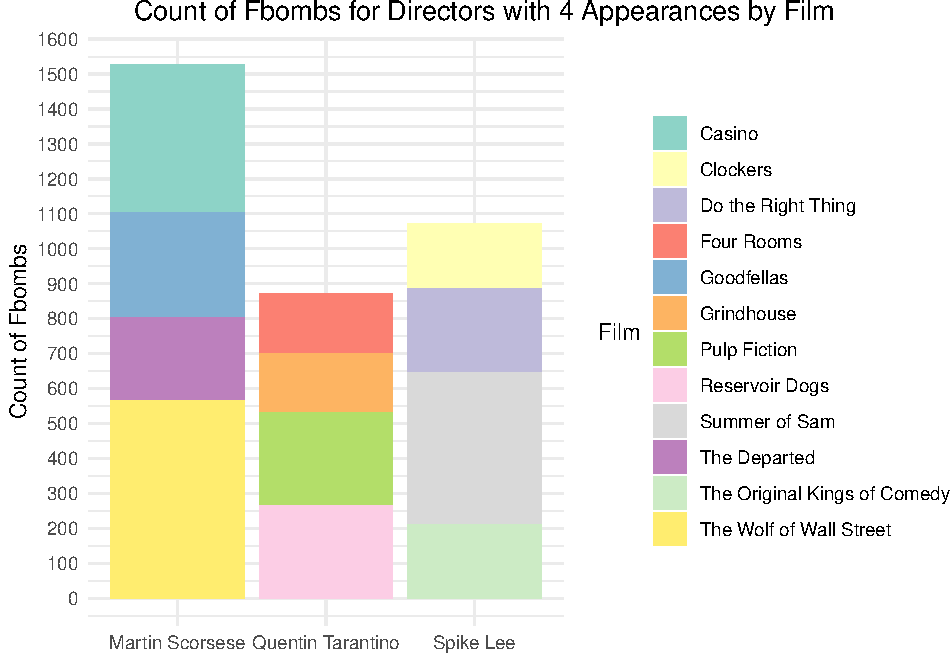
\includegraphics{project1.ethanpieniazekweb_files/figure-latex/unnamed-chunk-14-1} \end{center}

\emph{It was interesting to find that out of 132 observations there were
three directors that each had four films in the data. Martin Scorsese
had the film with the most f-bombs in the dataset (``The Wolf of Wall
Street) and Spike Lee has the film with the second most f-bombs in the
dataset (''Summer of Sam``). Quentin Tarantino had the lowest combined
f-bomb count for his four films when compared to Spike Lee's and Martin
Scorsese's totals (Martin surpassing Spike Lee by nearly 600 f-bombs!).
I found it particularly interesting that Tarantino had two pairs of
films in the data with very similar f-bomb totals.''Pulp Fiction" had
265 while ``Reservoir Dogs'' had 269 and ``Grindhouse'' had 169 while
``Four Rooms'' had 168. I wish I could have gotten around to watching
``Once Upon a Time in Hollywood'' again and while tallying the f-bombs
as I watched it to see how it compared to his other four films. If the
film ended up having greater than 150 f-bombs (highly likely in a nearly
three hour Tarantino film considering his past record) then Tarantino
would have been the single director with the most films that made the
list at five films total.}

\hypertarget{second-plot}{%
\section{Second Plot}\label{second-plot}}

\begin{Shaded}
\begin{Highlighting}[]
\NormalTok{complot <-}\StringTok{ }\KeywordTok{ggplot}\NormalTok{(filmsdata, }\KeywordTok{aes}\NormalTok{(}\DataTypeTok{x =} \KeywordTok{factor}\NormalTok{(quintileyr), }\DataTypeTok{y =}\NormalTok{ domesticgross)) }\OperatorTok{+}\StringTok{ }
\StringTok{    }\KeywordTok{geom_bar}\NormalTok{(}\DataTypeTok{stat =} \StringTok{"summary"}\NormalTok{, }\DataTypeTok{fun.y =} \StringTok{"mean"}\NormalTok{, }\KeywordTok{aes}\NormalTok{(}\DataTypeTok{fill =}\NormalTok{ comedy)) }\OperatorTok{+}\StringTok{ }
\StringTok{    }\KeywordTok{scale_y_continuous}\NormalTok{(}\DataTypeTok{name =} \StringTok{"Average Revenue in US Dollars"}\NormalTok{, }
        \DataTypeTok{labels =}\NormalTok{ scales}\OperatorTok{::}\NormalTok{comma, }\DataTypeTok{breaks =} \KeywordTok{seq}\NormalTok{(}\DataTypeTok{from =} \DecValTok{0}\NormalTok{, }\DataTypeTok{to =} \FloatTok{7e+07}\NormalTok{, }
            \DataTypeTok{by =} \FloatTok{5e+06}\NormalTok{)) }\OperatorTok{+}\StringTok{ }\KeywordTok{ggtitle}\NormalTok{(}\StringTok{"Average Domestic Box Office Sales per Quintile by Genre"}\NormalTok{) }\OperatorTok{+}\StringTok{ }
\StringTok{    }\KeywordTok{xlab}\NormalTok{(}\StringTok{"Quintile"}\NormalTok{) }\OperatorTok{+}\StringTok{ }\KeywordTok{ylab}\NormalTok{(}\StringTok{"Count of Fbombs"}\NormalTok{) }\OperatorTok{+}\StringTok{ }\KeywordTok{theme_minimal}\NormalTok{() }\OperatorTok{+}\StringTok{ }
\StringTok{    }\KeywordTok{theme}\NormalTok{(}\DataTypeTok{plot.title =} \KeywordTok{element_text}\NormalTok{(}\DataTypeTok{hjust =} \FloatTok{0.5}\NormalTok{)) }\OperatorTok{+}\StringTok{ }\KeywordTok{scale_fill_brewer}\NormalTok{(}\DataTypeTok{palette =} \StringTok{"Set3"}\NormalTok{) }\OperatorTok{+}\StringTok{ }
\StringTok{    }\KeywordTok{facet_wrap}\NormalTok{(}\OperatorTok{~}\NormalTok{comedy)}

\NormalTok{comedylabels <-}\StringTok{ }\KeywordTok{c}\NormalTok{(}\DataTypeTok{no =} \StringTok{"Non-comedy"}\NormalTok{, }\DataTypeTok{yes =} \StringTok{"Comedy"}\NormalTok{)}

\NormalTok{complot }\OperatorTok{+}\StringTok{ }\KeywordTok{facet_grid}\NormalTok{(. }\OperatorTok{~}\StringTok{ }\NormalTok{comedy, }\DataTypeTok{labeller =} \KeywordTok{labeller}\NormalTok{(}\DataTypeTok{comedy =}\NormalTok{ comedylabels)) }\OperatorTok{+}\StringTok{ }
\StringTok{    }\KeywordTok{theme}\NormalTok{(}\DataTypeTok{legend.position =} \StringTok{"none"}\NormalTok{) }\OperatorTok{+}\StringTok{ }\KeywordTok{scale_x_discrete}\NormalTok{(}\DataTypeTok{breaks =} \KeywordTok{c}\NormalTok{(}\StringTok{"[1978,1997]"}\NormalTok{, }
    \StringTok{"(1997,2000]"}\NormalTok{, }\StringTok{"(2000,2006]"}\NormalTok{, }\StringTok{"(2006,2012]"}\NormalTok{, }\StringTok{"(2012,2019]"}\NormalTok{), }
    \DataTypeTok{labels =} \KeywordTok{c}\NormalTok{(}\StringTok{"1978-97"}\NormalTok{, }\StringTok{"1998-00"}\NormalTok{, }\StringTok{"2001-06"}\NormalTok{, }\StringTok{"2007-12"}\NormalTok{, }\StringTok{"2013-19"}\NormalTok{)) }\OperatorTok{+}\StringTok{ }
\StringTok{    }\KeywordTok{theme}\NormalTok{(}\DataTypeTok{axis.text.x =} \KeywordTok{element_text}\NormalTok{(}\DataTypeTok{angle =} \DecValTok{27}\NormalTok{, }\DataTypeTok{vjust =} \FloatTok{0.5}\NormalTok{))}
\end{Highlighting}
\end{Shaded}

\begin{center}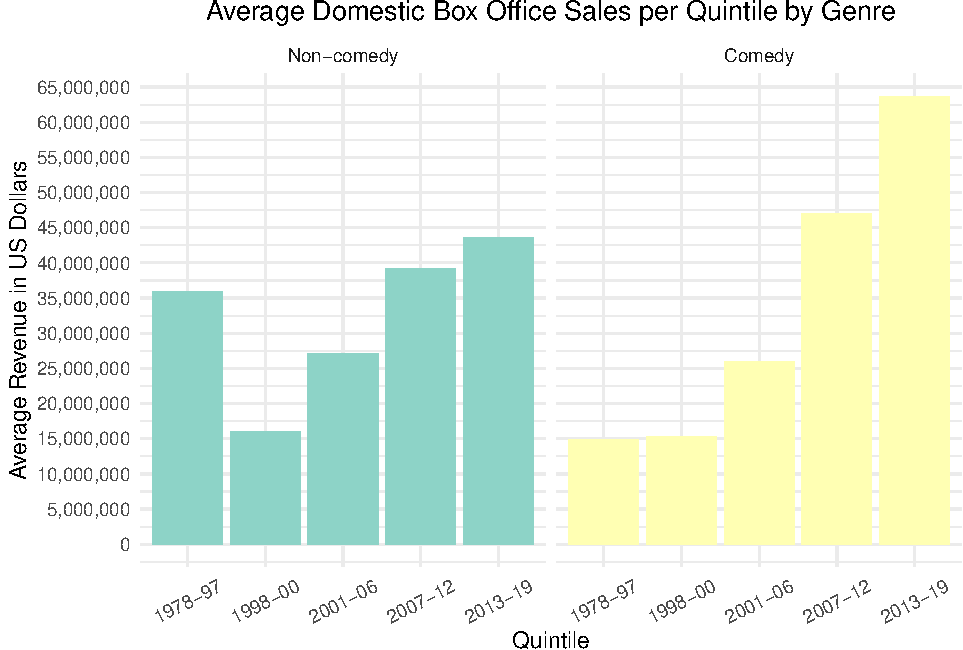
\includegraphics{project1.ethanpieniazekweb_files/figure-latex/unnamed-chunk-15-1} \end{center}

\emph{This plot shows how the comedies compare to the non-comedies when
average domestic box office sales is concerned, based on quintile. I
made the quintiles to better compare observations as otherwise it would
simply be a plot of each year's average revenue (in some cases just
being the revenue one movie brought in rather than a true average since
it was the only one for a particular year). Forming five quintiles from
the years made it more intuitive to see which range of years brought in
the most revenue for these highly vulgar movies. As one can see the
fifth quantile has the highest average revenue in both the comedy and
non-comedy groups. This may partly be due to the top 3 grossing films in
the dataset being from the fifth quartile (``22 Jump Street'',
``Straight Outta Compton'', and ``The Heat''), but making five quintiles
allows for a better assessment of average revenue than if one were to
divide the years into 10 quintiles for such a small dataset. The
non-comedies consisting of action films, dramas, crime films, etc. on
average did better in the box office than the comedies until after 2006.
Another interesting trend is that the average revenue for the
non-comedies in first quintile starts strong, but tapers off or remains
close to the first quintile in later years. The comedies on the other
hand always show a considerable increase in average revenue as the
quintiles proceed to 2013-2019, the quintile with highest revenue in the
comedy group as well as when compared to the non-comedies.}

\hypertarget{clustering}{%
\section{Clustering}\label{clustering}}

\begin{Shaded}
\begin{Highlighting}[]
\KeywordTok{library}\NormalTok{(cluster)}
\NormalTok{filmsclust <-}\StringTok{ }\NormalTok{filmsdata }\OperatorTok\StringTok{ }\KeywordTok{select}\NormalTok{(fbombs, minutes, domesticgross, }
\NormalTok{    fbombspermin)}
\NormalTok{sil_width <-}\StringTok{ }\KeywordTok{vector}\NormalTok{()}
\ControlFlowTok{for}\NormalTok{ (i }\ControlFlowTok{in} \DecValTok{2}\OperatorTok{:}\DecValTok{10}\NormalTok{) \{}
\NormalTok{    pam_fit <-}\StringTok{ }\KeywordTok{pam}\NormalTok{(filmsclust, }\DataTypeTok{k =}\NormalTok{ i)}
\NormalTok{    sil_width[i] <-}\StringTok{ }\NormalTok{pam_fit}\OperatorTok{$}\NormalTok{silinfo}\OperatorTok{$}\NormalTok{avg.width}
\NormalTok{\}}
\KeywordTok{ggplot}\NormalTok{() }\OperatorTok{+}\StringTok{ }\KeywordTok{geom_line}\NormalTok{(}\KeywordTok{aes}\NormalTok{(}\DataTypeTok{x =} \DecValTok{1}\OperatorTok{:}\DecValTok{10}\NormalTok{, }\DataTypeTok{y =}\NormalTok{ sil_width)) }\OperatorTok{+}\StringTok{ }\KeywordTok{scale_x_continuous}\NormalTok{(}\DataTypeTok{name =} \StringTok{"k"}\NormalTok{, }
    \DataTypeTok{breaks =} \DecValTok{1}\OperatorTok{:}\DecValTok{10}\NormalTok{)}
\end{Highlighting}
\end{Shaded}

\begin{center}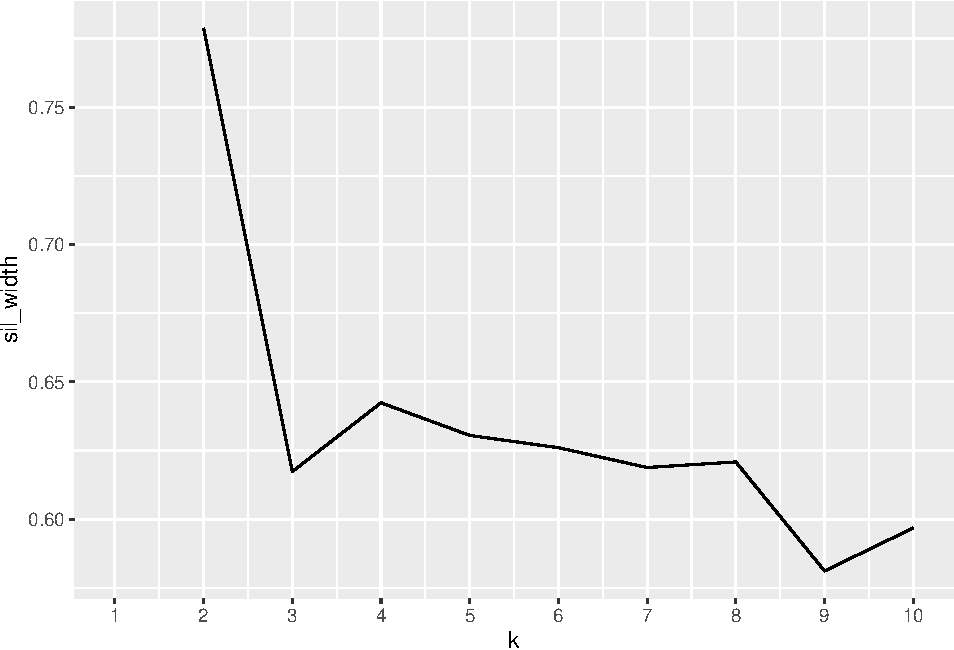
\includegraphics{project1.ethanpieniazekweb_files/figure-latex/unnamed-chunk-16-1} \end{center}

\begin{Shaded}
\begin{Highlighting}[]
\NormalTok{pamfilms <-}\StringTok{ }\KeywordTok{pam}\NormalTok{(filmsclust, }\DataTypeTok{k =} \DecValTok{2}\NormalTok{)}
\NormalTok{silpam <-}\StringTok{ }\KeywordTok{silhouette}\NormalTok{(pamfilms)}
\KeywordTok{plot}\NormalTok{(silpam)}
\end{Highlighting}
\end{Shaded}

\begin{center}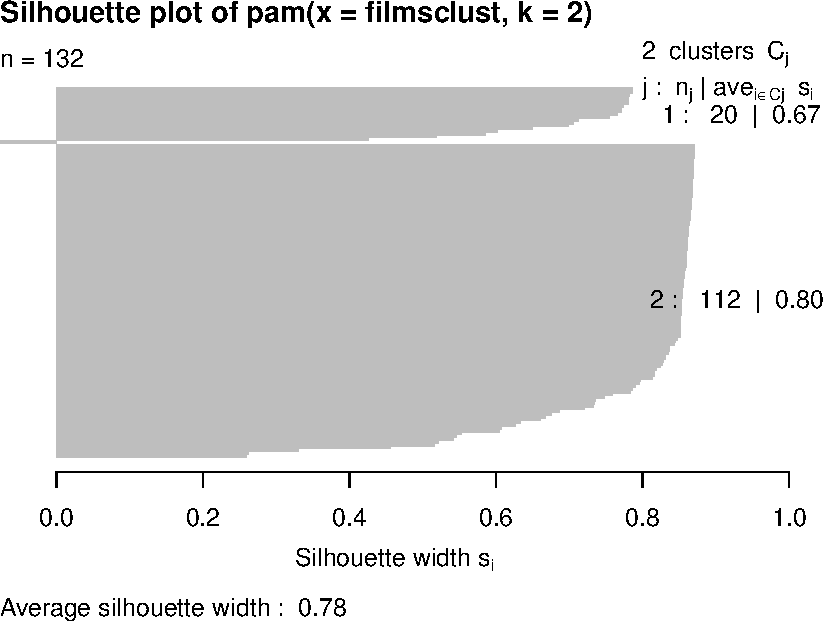
\includegraphics{project1.ethanpieniazekweb_files/figure-latex/unnamed-chunk-16-2} \end{center}

\begin{Shaded}
\begin{Highlighting}[]
\NormalTok{finalfilmsclust <-}\StringTok{ }\NormalTok{filmsdata }\OperatorTok\StringTok{ }\KeywordTok{mutate}\NormalTok{(}\DataTypeTok{cluster =} \KeywordTok{as.factor}\NormalTok{(pamfilms}\OperatorTok{$}\NormalTok{clustering))}
\KeywordTok{ggplot}\NormalTok{(finalfilmsclust, }\KeywordTok{aes}\NormalTok{(}\DataTypeTok{x =}\NormalTok{ domesticgross, }\DataTypeTok{y =}\NormalTok{ fbombspermin, }
    \DataTypeTok{color =}\NormalTok{ cluster)) }\OperatorTok{+}\StringTok{ }\KeywordTok{geom_point}\NormalTok{()}
\end{Highlighting}
\end{Shaded}

\begin{center}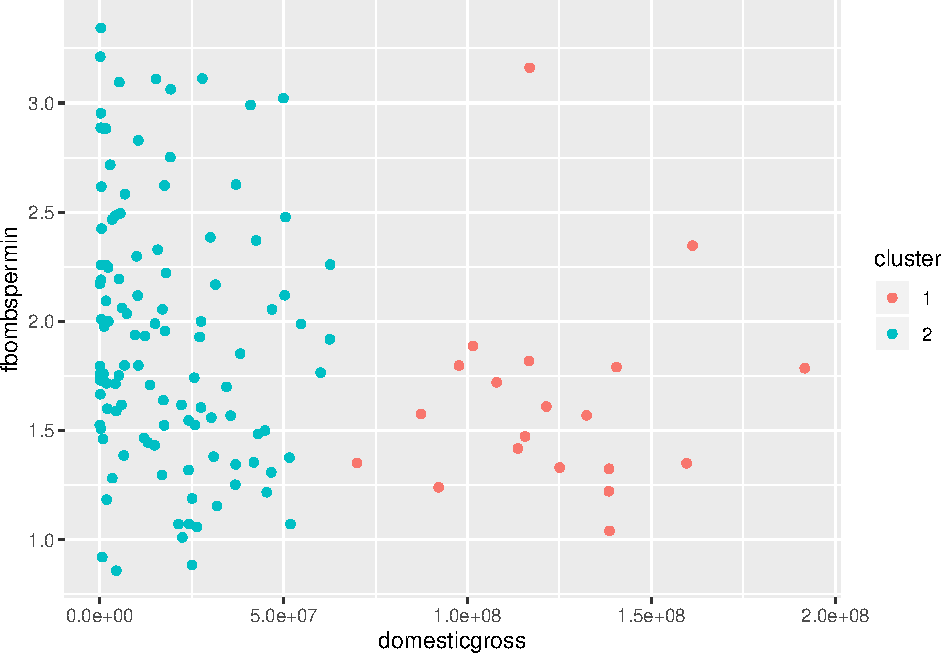
\includegraphics{project1.ethanpieniazekweb_files/figure-latex/unnamed-chunk-16-3} \end{center}

\begin{Shaded}
\begin{Highlighting}[]
\KeywordTok{library}\NormalTok{(GGally)}
\NormalTok{finalfilmsclust }\OperatorTok\StringTok{ }\KeywordTok{select}\NormalTok{(fbombs, minutes, domesticgross, fbombspermin, }
\NormalTok{    cluster) }\OperatorTok\StringTok{ }\KeywordTok{ggpairs}\NormalTok{(}\DataTypeTok{columns =} \DecValTok{1}\OperatorTok{:}\DecValTok{4}\NormalTok{, }\KeywordTok{aes}\NormalTok{(}\DataTypeTok{color =}\NormalTok{ cluster))}
\end{Highlighting}
\end{Shaded}

\begin{center}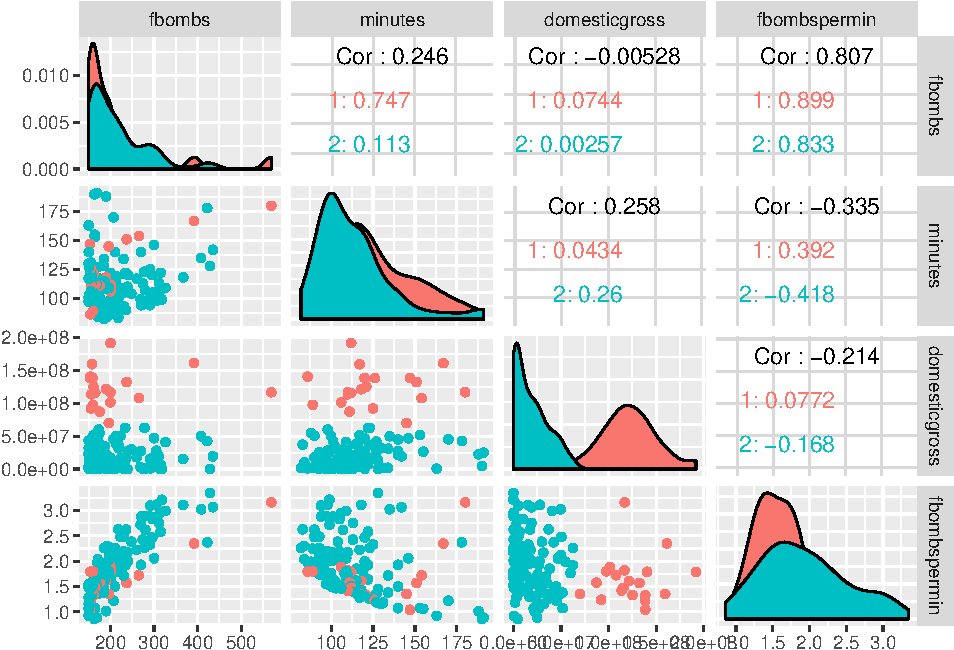
\includegraphics{project1.ethanpieniazekweb_files/figure-latex/unnamed-chunk-16-4} \end{center}

\emph{After performing PAM and kmeans clustering, I found out the two
clustered the data quite differently. I went with PAM as the clusters
seemed more distinct for the variables at hand. After making a new
dataframe only containing the numeric variables of interest (fbombs,
minutes, domesticgross, and fbombspermin), sil\_width showed it made the
most sense to cluster into two after analysis of the plot.When viewing
the separate silhouette plot, PAM clustering showed there was strong
structure (average silhouette width = 0.78) to be found between the two
clusters, so most of the values belonged to the clusters they were
assigned.}

\emph{The ggpairs package provided a nice cohesive summary all in one
chart, separated into several boxes based on information about
correlations between two variables concerning the clusters. The the
number of f-bombs in a film was shown to almost have much no correlation
to the domestic box office sales. So increased cursing in a film did not
correlate with increased revenue or vise versa, which makes sense since
all these films are rated R and the target audience is greatly limited
to adults. The highest positive correlation was seen between
`fbombspermin' and `fbombs'. Both cluster 1 and 2 exhibited this with
values at 0.89 and 0.83 respectively. This also makes sense because the
more f-bombs a film has is going to directly correlate with more f-bombs
that film has per minute.}

\emph{Taking information gathered from the ggpairs analysis, plotting
with ggplot based on x = `domesticgross' and y = `fbombspermin' was
performed as the clusters appeared the most separated and the two
variables compared the most relevant. After looking at the ggplot as
well as the data itself (arranging descending by variable) for the
dataframe with the now included clusters it was apparent that clustering
was largely based on how well the film did at the box office. Having a
relatively small dataset made understanding and comprehension the data
very manageable, as direct films could easily be found from cluster 2.
It was really neat to find out with exceptions that most of the top
grossing films ended up having only a moderate amount of f-bombs per
minute when compared to many from cluster 2. Of course outliers such as
``The Wolf of Wall Street'' and ``Straight Outta Compton'' ended up
doing exceptionally well despite the frequency of the word, but these
are the only 2 out of 20 that showed this difference in cluster 1. Of
course all 132 of these films had tons of vulgar language as they were
the ones that made the ``List of films that most frequently use the
word''f\$\#\%", but nevertheless it was a fun time exploring the several
differences and similarities between them.}

\end{document}
